\begin{mydef}{Experiment}{def_exp}
  Im Zuge dieser Arbeit impliziert der Begriff „Wirtschaftsinformatik“ die Betrachtung (konstruierter) IT-Artefakte ausschließlich in Form softwareseitiger Anwendungssysteme.
  This theorem is numbered with  \ref{def:def_exp} and is given on page \pageref{def:def_exp}.
\end{mydef}



%%Einbindung der Grafiken rotiert %% 
 
 \begin{figure}[h]
 \centering
 \resizebox{\textwidth}{!}{%
 \IfFileExists{../../_preamble/check_file.tex}% prüfen aus welcher datei der aufruf stattfindet
{%
\providecommand{\myPath}{../../}% file exists=true: befinde mich im unterverzeichnis
}%
{%
\providecommand{\myPath}{}% file exists=false: befinde mich im root_verzeichnis
}%
\documentclass[tikz]{standalone}
%% läd standalone-klasse mit tikz-argument
%//Tikzbibliotheken\\%
\usetikzlibrary{						% Bibliotheken zur direkten Einbindung in TIKZEdt
arrows, 
fit,
shapes.geometric, 
matrix,
calc,
decorations.markings,
decorations.pathreplacing,
decorations.pathmorphing,
backgrounds,
shadings, 
shadows,
positioning,
mindmap,
trees,
datavisualization
}%% diverse tikz-bibliotheken
%%Font etc.%%
\usepackage{lmodern}					% OK, Latin Modern font,											check: 25.08.18
\usepackage{xcolor} 					% OK, Definieren und Nutzen von versch. Farben						check: 25.08.18
\usepackage{graphicx}					% OK, Bereitstellen von \includegraphics							check: 25.08.18

%%Forest%%
\usepackage{forest}						% OK, Baumdarstellung aus dem linguistischen Bereich				check: 25.08.18
\useforestlibrary{edges}

%%Venndiagramm%%
\usepackage{venndiagram}				% OK, Definieren und Darstellen von Venndiagrammen					check: 25.08.18

%%Tabellen%%
\usepackage{booktabs}					% OK, Schönere Tabellen ohne vertikale Linien \toprule etc.			check: 25.08.18
\usepackage{tabularx}					% OK, Weiterer Spaltentyp passt Tabellenbreite  automatisch an		check: 25.08.18
\usepackage{multirow}					% OK, Zellenspannung über mehrere Zeilen							check: 25.08.18
%\usepackage{makecell}					% OK, Tabellenlayout (Tabaellenheader) ähnlich \multirow			check: 25.08.18
\usepackage{tablefootnote}				% OK, Fußnoten in Tabellen (\footnote funktioniert nicht)			check: 25.08.18
\usepackage{array} 						% OK, Erstellen eigener Columntypen in Tabellenumgebungen			check: 25.08.18

%%Grafiken und Plots%%
\usepackage{tikz} 						% OK, Natives zeichnen in Latex ,									check: 25.08.18
\usepackage{tikz-cd} 					% OK, Erstellen von kommutativen Diagrammen in Tikz,				check: 25.08.18
\usepackage{pgfplots}					% OK, Plotten von Daten,											check: 25.08.18
\pgfplotsset{compat=newest}				% OK, Einstellen der Kompatibilitätsversion,						check: 25.08.18
\usepackage{pgfplotstable}				% OK, Plotten und schreiben von Daten in Tabellen,					check: 25.08.18
\usepackage{pgfcalendar} 				% OK, Umrechnen von Datumskoordinaten,								check: 25.08.18
\usepgfplotslibrary{dateplot}			% OK, Plotten von Datumskoordinaten,								check: 25.08.18
\usepgfplotslibrary{units}				% OK, Darstellen von Einheiten als Achsenlabel,						check: 25.08.18%% nur laden wenn weitere graphic pakete benötigt werden (tabellen, pgfplot,...)
%%define tikz-stlyes here, colours etc.
\tikzset{
block_phantom/.style={block_normal, draw=red, fill=none},
block_phantom/.style={block_normal, draw=blue, fill=none}
}
%\tikzstyle{block_phantom}=[block_normal, draw=red, fill=none]%% tikz-styles, farben etc.
\begin{document}
\begin{forest}
for tree={grow=south},forked edges,
[Experimente zum Thema Kreativität in der Wirtschatfsinformatik
    [ Veröffentlichung
        [<1990]
        [<2000]
        [<2010]
        [>2010]
    ]
    [Aufgabenart
        [Generierung
            [Probandenrelevant]
            [Nicht Probandenrelevant]
        ]
        [Selektion
            [Probandenrelevant]
            [Nicht Probandenrelevant]
        ]
    ]
    [,phantom
        [,phantom
            [,phantom
                [test
                    [test1] [test2 [test3]]
                ]
            ]
        ]
    ]
    [Teilnehmermotivation
        [Bezahlung
            [>10 Euro]
            [<=10 Euro]
        ]
        [Leistungspunkte]
        [Teilnehmerrelevanz]
    ]
    [Kontrolle von Störgrößen
    [4
            [Gruppe6]
        ]
        [Gruppe5]
    ]
    [Gruppe 4
    [4
            [Gruppe6]
        ]
        [Gruppe5 [Gruppe4[Gruppe8[7[0[Gruppe4]]]]]]
    ]
    [Gruppe 5
    [Gruppe4
            [Gruppe6]
        ]
        [5]
    ]
    [Gruppe 6
    [Gruppe4
            [Gruppe6]
        ]
        [Gruppe5]
    ]
]
\end{forest}

\end{document}
%
 }
 \caption{}
 \end{figure}

 
\begin{sidewaysfigure}
    \centering
    \resizebox{\textwidth}{!}{%
    \IfFileExists{../../_preamble/check_file.tex}% prüfen aus welcher datei der aufruf stattfindet
{%
\providecommand{\myPath}{../../}% file exists=true: befinde mich im unterverzeichnis
}%
{%
\providecommand{\myPath}{}% file exists=false: befinde mich im root_verzeichnis
}%
\documentclass[tikz]{standalone}
%% läd standalone-klasse mit tikz-argument
%//Tikzbibliotheken\\%
\usetikzlibrary{						% Bibliotheken zur direkten Einbindung in TIKZEdt
arrows, 
fit,
shapes.geometric, 
matrix,
calc,
decorations.markings,
decorations.pathreplacing,
decorations.pathmorphing,
backgrounds,
shadings, 
shadows,
positioning,
mindmap,
trees,
datavisualization
}%% diverse tikz-bibliotheken
%%Font etc.%%
\usepackage{lmodern}					% OK, Latin Modern font,											check: 25.08.18
\usepackage{xcolor} 					% OK, Definieren und Nutzen von versch. Farben						check: 25.08.18
\usepackage{graphicx}					% OK, Bereitstellen von \includegraphics							check: 25.08.18

%%Forest%%
\usepackage{forest}						% OK, Baumdarstellung aus dem linguistischen Bereich				check: 25.08.18
\useforestlibrary{edges}

%%Venndiagramm%%
\usepackage{venndiagram}				% OK, Definieren und Darstellen von Venndiagrammen					check: 25.08.18

%%Tabellen%%
\usepackage{booktabs}					% OK, Schönere Tabellen ohne vertikale Linien \toprule etc.			check: 25.08.18
\usepackage{tabularx}					% OK, Weiterer Spaltentyp passt Tabellenbreite  automatisch an		check: 25.08.18
\usepackage{multirow}					% OK, Zellenspannung über mehrere Zeilen							check: 25.08.18
%\usepackage{makecell}					% OK, Tabellenlayout (Tabaellenheader) ähnlich \multirow			check: 25.08.18
\usepackage{tablefootnote}				% OK, Fußnoten in Tabellen (\footnote funktioniert nicht)			check: 25.08.18
\usepackage{array} 						% OK, Erstellen eigener Columntypen in Tabellenumgebungen			check: 25.08.18

%%Grafiken und Plots%%
\usepackage{tikz} 						% OK, Natives zeichnen in Latex ,									check: 25.08.18
\usepackage{tikz-cd} 					% OK, Erstellen von kommutativen Diagrammen in Tikz,				check: 25.08.18
\usepackage{pgfplots}					% OK, Plotten von Daten,											check: 25.08.18
\pgfplotsset{compat=newest}				% OK, Einstellen der Kompatibilitätsversion,						check: 25.08.18
\usepackage{pgfplotstable}				% OK, Plotten und schreiben von Daten in Tabellen,					check: 25.08.18
\usepackage{pgfcalendar} 				% OK, Umrechnen von Datumskoordinaten,								check: 25.08.18
\usepgfplotslibrary{dateplot}			% OK, Plotten von Datumskoordinaten,								check: 25.08.18
\usepgfplotslibrary{units}				% OK, Darstellen von Einheiten als Achsenlabel,						check: 25.08.18%% nur laden wenn weitere graphic pakete benötigt werden (tabellen, pgfplot,...)
%%define tikz-stlyes here, colours etc.
\tikzset{
block_phantom/.style={block_normal, draw=red, fill=none},
block_phantom/.style={block_normal, draw=blue, fill=none}
}
%\tikzstyle{block_phantom}=[block_normal, draw=red, fill=none]%% tikz-styles, farben etc.
\begin{document}
\begin{forest}
for tree={grow=south},forked edges,
[Experimente zum Thema Kreativität in der Wirtschatfsinformatik
    [ Veröffentlichung
        [<1990]
        [<2000]
        [<2010]
        [>2010]
    ]
    [Aufgabenart
        [Generierung
            [Probandenrelevant]
            [Nicht Probandenrelevant]
        ]
        [Selektion
            [Probandenrelevant]
            [Nicht Probandenrelevant]
        ]
    ]
    [,phantom
        [,phantom
            [,phantom
                [test
                    [test1] [test2 [test3]]
                ]
            ]
        ]
    ]
    [Teilnehmermotivation
        [Bezahlung
            [>10 Euro]
            [<=10 Euro]
        ]
        [Leistungspunkte]
        [Teilnehmerrelevanz]
    ]
    [Kontrolle von Störgrößen
    [4
            [Gruppe6]
        ]
        [Gruppe5]
    ]
    [Gruppe 4
    [4
            [Gruppe6]
        ]
        [Gruppe5 [Gruppe4[Gruppe8[7[0[Gruppe4]]]]]]
    ]
    [Gruppe 5
    [Gruppe4
            [Gruppe6]
        ]
        [5]
    ]
    [Gruppe 6
    [Gruppe4
            [Gruppe6]
        ]
        [Gruppe5]
    ]
]
\end{forest}

\end{document}
%
    }
    \caption{ Here is a caption of the figure which is so long that 
      it has to be wrapped over multiple lines, but should 
      not exceed the width (height after the rotation) of the image.}
    \label{fig:awesome_image}
\end{sidewaysfigure}

 
\begin{figure}[ht]
  \begin{adjustbox}{addcode={\begin{minipage}{\width}}{\caption{%
      Here is a caption of the figure which is so long that 
      it has to be wrapped over multiple lines, but should 
      not exceed the width (height after the rotation) of the image.
      }\end{minipage}},rotate=90,center}
      \resizebox{\textheight}{!}{%
      \IfFileExists{../../_preamble/check_file.tex}% prüfen aus welcher datei der aufruf stattfindet
{%
\providecommand{\myPath}{../../}% file exists=true: befinde mich im unterverzeichnis
}%
{%
\providecommand{\myPath}{}% file exists=false: befinde mich im root_verzeichnis
}%
\documentclass[tikz]{standalone}
%% läd standalone-klasse mit tikz-argument
%//Tikzbibliotheken\\%
\usetikzlibrary{						% Bibliotheken zur direkten Einbindung in TIKZEdt
arrows, 
fit,
shapes.geometric, 
matrix,
calc,
decorations.markings,
decorations.pathreplacing,
decorations.pathmorphing,
backgrounds,
shadings, 
shadows,
positioning,
mindmap,
trees,
datavisualization
}%% diverse tikz-bibliotheken
%%Font etc.%%
\usepackage{lmodern}					% OK, Latin Modern font,											check: 25.08.18
\usepackage{xcolor} 					% OK, Definieren und Nutzen von versch. Farben						check: 25.08.18
\usepackage{graphicx}					% OK, Bereitstellen von \includegraphics							check: 25.08.18

%%Forest%%
\usepackage{forest}						% OK, Baumdarstellung aus dem linguistischen Bereich				check: 25.08.18
\useforestlibrary{edges}

%%Venndiagramm%%
\usepackage{venndiagram}				% OK, Definieren und Darstellen von Venndiagrammen					check: 25.08.18

%%Tabellen%%
\usepackage{booktabs}					% OK, Schönere Tabellen ohne vertikale Linien \toprule etc.			check: 25.08.18
\usepackage{tabularx}					% OK, Weiterer Spaltentyp passt Tabellenbreite  automatisch an		check: 25.08.18
\usepackage{multirow}					% OK, Zellenspannung über mehrere Zeilen							check: 25.08.18
%\usepackage{makecell}					% OK, Tabellenlayout (Tabaellenheader) ähnlich \multirow			check: 25.08.18
\usepackage{tablefootnote}				% OK, Fußnoten in Tabellen (\footnote funktioniert nicht)			check: 25.08.18
\usepackage{array} 						% OK, Erstellen eigener Columntypen in Tabellenumgebungen			check: 25.08.18

%%Grafiken und Plots%%
\usepackage{tikz} 						% OK, Natives zeichnen in Latex ,									check: 25.08.18
\usepackage{tikz-cd} 					% OK, Erstellen von kommutativen Diagrammen in Tikz,				check: 25.08.18
\usepackage{pgfplots}					% OK, Plotten von Daten,											check: 25.08.18
\pgfplotsset{compat=newest}				% OK, Einstellen der Kompatibilitätsversion,						check: 25.08.18
\usepackage{pgfplotstable}				% OK, Plotten und schreiben von Daten in Tabellen,					check: 25.08.18
\usepackage{pgfcalendar} 				% OK, Umrechnen von Datumskoordinaten,								check: 25.08.18
\usepgfplotslibrary{dateplot}			% OK, Plotten von Datumskoordinaten,								check: 25.08.18
\usepgfplotslibrary{units}				% OK, Darstellen von Einheiten als Achsenlabel,						check: 25.08.18%% nur laden wenn weitere graphic pakete benötigt werden (tabellen, pgfplot,...)
%%define tikz-stlyes here, colours etc.
\tikzset{
block_phantom/.style={block_normal, draw=red, fill=none},
block_phantom/.style={block_normal, draw=blue, fill=none}
}
%\tikzstyle{block_phantom}=[block_normal, draw=red, fill=none]%% tikz-styles, farben etc.
\begin{document}
\begin{forest}
for tree={grow=south},forked edges,
[Experimente zum Thema Kreativität in der Wirtschatfsinformatik
    [ Veröffentlichung
        [<1990]
        [<2000]
        [<2010]
        [>2010]
    ]
    [Aufgabenart
        [Generierung
            [Probandenrelevant]
            [Nicht Probandenrelevant]
        ]
        [Selektion
            [Probandenrelevant]
            [Nicht Probandenrelevant]
        ]
    ]
    [,phantom
        [,phantom
            [,phantom
                [test
                    [test1] [test2 [test3]]
                ]
            ]
        ]
    ]
    [Teilnehmermotivation
        [Bezahlung
            [>10 Euro]
            [<=10 Euro]
        ]
        [Leistungspunkte]
        [Teilnehmerrelevanz]
    ]
    [Kontrolle von Störgrößen
    [4
            [Gruppe6]
        ]
        [Gruppe5]
    ]
    [Gruppe 4
    [4
            [Gruppe6]
        ]
        [Gruppe5 [Gruppe4[Gruppe8[7[0[Gruppe4]]]]]]
    ]
    [Gruppe 5
    [Gruppe4
            [Gruppe6]
        ]
        [5]
    ]
    [Gruppe 6
    [Gruppe4
            [Gruppe6]
        ]
        [Gruppe5]
    ]
]
\end{forest}

\end{document}
%
      }
  \end{adjustbox}
\end{figure}
 
 
\begin{figure}[ht]
  \begin{adjustbox}{addcode={\begin{minipage}{\width}}{\caption{%
      Here is a caption of the figure which is so long that 
      it has to be wrapped over multiple lines, but should 
      not exceed the width (height after the rotation) of the image.
      }\end{minipage}},rotate=90,center}
      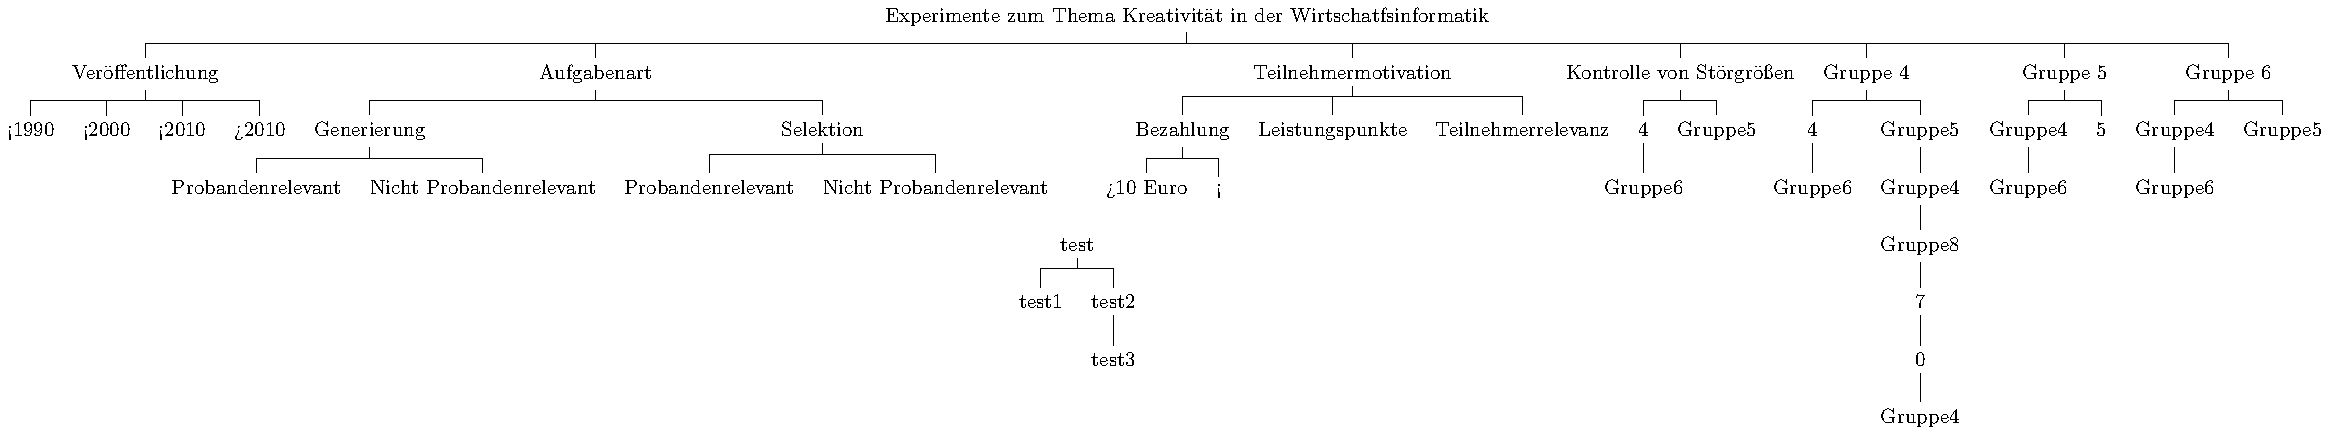
\includegraphics[width=\textheight]{_img/_forest/block_experiment.pdf}%
  \end{adjustbox}
\end{figure}
